\clearpage
\VerdierPhysicalPageAnchor{0237}%
\begingroup\small\setlength{\parskip}{0pt}\setlength{\emergencystretch}{1.5em}
\setlength{\abovedisplayskip}{4pt plus 2pt minus 2pt}%
\setlength{\belowdisplayskip}{4pt plus 2pt minus 2pt}%

\VerdierSemanticAnchor{ch4d-4-3-2}
\noindent\textbf{命題 4.3.2.}\quad
\textit{$X$ を $\operatorname{comp}(\mathcal A)$ の対象、
$\bigl(X(p,q),\delta(p,q,r)\bigr)$ を $X$ に付随する第二スペクトル対象、
$H\colon D(\mathcal A)\longrightarrow\mathcal A$ を標準コホモロジー的関手とする。}

\VerdierSemanticAnchor{ch4d-4-3-2-a}
\noindent\textit{a) 整数が $r<p$ または $r\geq q$ を満たすとき、
$H^r\bigl(X(p,q)\bigr)=0$ である。}

\VerdierSemanticAnchor{ch4d-4-3-2-b}
\noindent\textit{b) $r$ を整数とする。
$\mathcal{F}\ell_1(\widetilde{\mathbb Z})$ の元 $(p,q)$ で $p\leq r<q$ を
満たすものごとに、一意な同型}
\[
i_{p,q}^r(X)\colon H^r(X)\xrightarrow{\sim}H^r\bigl(X(p,q)\bigr)
\]
\noindent\textit{が存在し、$i_{-\infty,+\infty}^r(X)$ は恒等射である。
さらに、$(p,q)$ と $(p',q')$ が $p\leq p'$、$q\leq q'$、$p\leq r<q$、
$p'\leq r<q'$ を満たすとき、次の図式は可換である：}

\VerdierSemanticAnchor{ch4d-4-3-2-b-diagram}
\begin{center}
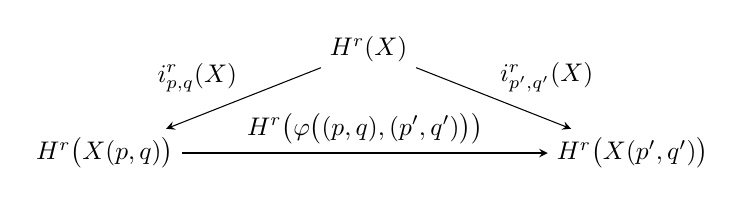
\begin{tikzpicture}[>=stealth,line width=.38pt,x=2.35cm,y=1.15cm,
  scale=.92,transform shape]
  \node (HX)  at (1.55,1.25) {$H^r(X)$};
  \node (Hpq) at (0,0) {$H^r\bigl(X(p,q)\bigr)$};
  \node (Hpp) at (3.10,0) {$H^r\bigl(X(p',q')\bigr)$};
  \draw[->] (HX) -- node[above left=-1pt] {$i_{p,q}^r(X)$} (Hpq);
  \draw[->] (HX) -- node[above right=-1pt] {$i_{p',q'}^r(X)$} (Hpp);
  \draw[->] (Hpq) -- node[above]
    {$H^r\!\left(\varphi\bigl((p,q),(p',q')\bigr)\right)$} (Hpp);
\end{tikzpicture}
\end{center}

\VerdierSemanticAnchor{ch4d-4-3-2-c}
\noindent\textit{c) $m\colon X\longrightarrow Y$ を
$\operatorname{comp}(\mathcal A)$ の射とし、}
\[
m(p,q)\colon X(p,q)\longrightarrow Y(p,q)
\]
\noindent\textit{を、付随する第二スペクトル対象の間の対応する射とする。
$\mathcal{F}\ell_1(\widetilde{\mathbb Z})$ の任意の元 $(p,q)$ と、
$p\leq r<q$ を満たす任意の整数 $r$ に対し、次の図式は可換である：}

\VerdierSemanticAnchor{ch4d-4-3-2-c-diagram}
\begin{center}
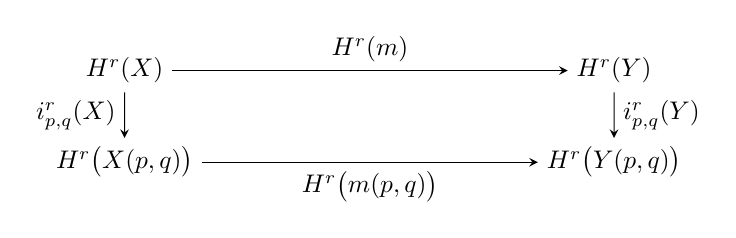
\begin{tikzpicture}[>=stealth,line width=.38pt,x=2.55cm,y=1.10cm,
  scale=.92,transform shape]
  \node (HX)  at (0,1.15) {$H^r(X)$};
  \node (HY)  at (2.65,1.15) {$H^r(Y)$};
  \node (Hpq) at (0,0) {$H^r\bigl(X(p,q)\bigr)$};
  \node (HpY) at (2.65,0) {$H^r\bigl(Y(p,q)\bigr)$};
  \draw[->] (HX) -- node[above] {$H^r(m)$} (HY);
  \draw[->] (Hpq) -- node[below] {$H^r\bigl(m(p,q)\bigr)$} (HpY);
  \draw[->] (HX) -- node[left] {$i_{p,q}^r(X)$} (Hpq);
  \draw[->] (HY) -- node[right] {$i_{p,q}^r(Y)$} (HpY);
\end{tikzpicture}
\end{center}

\noindent この命題は定義から直ちに従う。

\VerdierSemanticAnchor{ch4d-4-3-3}
\medskip\noindent\textbf{系 4.3.3.}\quad
\textit{第二標準スペクトル対象関手 (4.3.1) は、標準関手}
\[
\operatorname{comp}(\mathcal A)\longrightarrow D(\mathcal A).
\]
\noindent\textit{を通して一意に分解する。}

\VerdierSemanticAnchor{ch4d-4-3-3-proof}
実際、(4.3.2) により、この関手は擬同型 $m\colon X\longrightarrow Y$ を
スペクトル対象の同型に移す。したがってこの系は (1.3.5) から従う。
\endgroup
